\section{Experimental Evaluation}
\label{sec:experiments}

%%SL.5.24: For the sake of space, I think we can cut this and the subsection headings, and things are still mostly readable.
%The goal of our empirical evaluation is to study and compare the performance of CQL to prior offline RL methods on a wide range of domains and dataset compositions. We evaluate CQL along  multiple axes: the complexity of the underlying control problem, the way that the offline data is collected, and with both low-dimensional state and high-dimensional image inputs. 

% Additionally, we also evaluate CQL as an off-policy evaluation (OPE) method on the high-dimensional MuJoCo benchmark tasks, which typically pose a major challenge for modern OPE methods~\citep{nachum2019dualdice}. 

% Finally, we aim to analyze different components of CQL, highlighting the significance and empirical effects of the different design choices discussed in Section~\ref{sec:framework}.

%\subsection{Offline RL in Continuous Control Domains}
We compare CQL to prior offline RL methods on a range of domains and dataset compositions, including continuous and discrete action spaces, state observations of varying dimensionality, and high-dimensional image inputs. We first evaluate actor-critic CQL, using CQL($\mathcal{H}$) from Algorithm~\ref{alg:practical_alg}, on continuous control datasets from the D4RL benchmark~\citep{d4rl}.
We compare to: prior offline RL methods that use a policy constraint -- BEAR~\citep{kumar2019stabilizing} and BRAC~\citep{wu2019behavior}; SAC~\citep{haarnoja}, an off-policy actor-critic method that we adapt to offline setting; and behavioral cloning (BC). {The code and instructions for reproducing our latest results in jax can be found at: \url{https://github.com/young-geng/JaxCQL}. Please refer to this repository and the latest D4RL for future comparisons. D4RL-v0 is deprecated.}
% We also ran AlgeaDICE~\citep{nachum2019algaedice}, a method that uses a state-marginal constraint, using code released by the authors, but were unable to get it to improve over a random initialization on any of the tasks, as learning was unstable and diverged quickly, and we provide these learning curves in Appendix~\ref{app:additional_results}.
%%SL.5.24: For AlgeaDICE, I still think these sentences are damn awkward. If you really want to have this, maybe rephrase more briefly: We also attempted to run AlgeaDICE~\citep{} on these tasks, but were unable to obtain reasonable results with the authors' code (more details in Appendix~\ref{app:additional_results}). [I would also recommend omitting this sentence in the arxiv and only including it in the submission copy for the reviewers!]
% done, removed
%%SL.5.11: Could we add a comparison to AWR? I feel like this would not only make the results more complete, but also help to "legitimize" the viability of AWR as an offline RL algorithm. I think many readers of the original paper might have missed that AWR is also a good offline RL method, and by not comparing to it here, we in some sense reinforce that notion.
%%AK.5.13: TODO in the D4RL paper


\begin{table*}[h]
\captionsetup{font=small}
\centering
%\scriptsize
\fontsize{9}{9}\selectfont

\begin{tabular}{l|r|r|r|r|r||r}
\hline
\textbf{Task Name} & \textbf{SAC} & \textbf{BC} & \textbf{BEAR} & \textbf{BRAC-p} & \textbf{BRAC-v} & \textbf{CQL($\mathcal{H}$)}\\ \hline
% halfcheetah-random &  30.5 & 2.1 & 25.5 & 23.5 & 28.1 & \textbf{35.4} \\
% hopper-random & \textbf{11.3} & 9.8 & 9.5 & \textbf{11.1} & \textbf{12.0} & \textbf{10.8}\\
% walker2d-random & 4.1 & 1.6 & \textbf{6.7} & 0.8 & 0.5 & \textbf{7.0}\\ \hline
halfcheetah-medium-v2 & -4.3 & 42.6 & 38.6 & {44.0} & {51} & {48.4 $\pm$ 0.3}\\
walker2d-medium-v2 & 0.9 & 75.3  & 33.2 & 72.7 & {81.3} & {82.0 $\pm$ 1.0}\\
hopper-medium-v2 & 0.8 & 52.9 & 47.6 & 31.2 & {86.6} & {71.8 $\pm$ 2.5}\\ \hline
% halfcheetah-expert & -1.9 & \textbf{107.0} & \textbf{108.2} & 3.8 & -1.1 & {104.8}\\
% hopper-expert & 0.7 & \textbf{109.0} & \textbf{110.3} & 6.6 & 3.7 & \textbf{109.9} \\
% walker2d-expert & -0.3 & \textbf{125.7} & 106.1 & -0.2 & -0.0 & \textbf{121.6} \\ \hline
halfcheetah-medium-expert-v2 & 1.8 & 55.2 & 51.7 & 43.8 & 44.0 & {87.3 $\pm$ 0.2}\\
walker2d-medium-expert-v2 & 1.9 & 52.5 & 10.8 & -0.3 & {111.6} & {106.1 $\pm$ 7.2}\\
hopper-medium-expert-v2 & 1.6 & 107.5 & 4.0 & 1.1 & 79.0 & {109.2 $\pm$ 3.6}\\ \hline
halfcheetah-medium-replay-v2 & -2.4 & 36.6 & 36.2 & {47.6} & {45.3} & {47.0 $\pm$ 0.2} \\
hopper-medium-replay-v2 & 3.5 & 18.1 & 25.3 & 0.7 & {96.2} & {93.8 $\pm$ 2.8}\\
walker2d-medium-replay-v2 & 1.9 & 26.0 & 10.8 & -0.3 & {85.0} & {86.2 $\pm$ 0.2}\\
\hline
\textbf{Total} & 5.7 & 466.7 & - & - & 680.0 & \textbf{731.8}\\
\hline
\end{tabular}
\vspace{0.05cm}
\caption{\label{table:mujoco}{\small Performance of CQL($\mathcal{H}$) and prior methods on gym domains from D4RL, on the normalized return metric, averaged over 3 seeds. Note that CQL performs similarly or better than the best prior method with simple datasets, and outperforms prior methods with complex distributions (``--medium-replay'', ``--medium-expert'').}}
\normalsize
\vspace{-10pt}
\end{table*}



% \begin{table*}[h]
% \captionsetup{font=small}
% \centering
% %\scriptsize
% \fontsize{8}{8}\selectfont

% \begin{tabular}{l|r|r|r|r|r||r}
% \hline
% \textbf{Task Name} & \textbf{SAC} & \textbf{BC} & \textbf{BEAR} & \textbf{BRAC-p} & \textbf{BRAC-v} & \textbf{CQL($\mathcal{H}$)}\\ \hline
% % halfcheetah-random &  30.5 & 2.1 & 25.5 & 23.5 & 28.1 & \textbf{35.4} \\
% % hopper-random & \textbf{11.3} & 9.8 & 9.5 & \textbf{11.1} & \textbf{12.0} & \textbf{10.8}\\
% % walker2d-random & 4.1 & 1.6 & \textbf{6.7} & 0.8 & 0.5 & \textbf{7.0}\\ \hline
% halfcheetah-medium-v2 & -4.3 & 42.6 & 38.6 & \textbf{44.0} & \textbf{51} & {46.1}\\
% walker2d-medium-v2 & 0.9 & 75.3  & 33.2 & 72.7 & \textbf{81.3} & {74.5}\\
% hopper-medium-v2 & 0.8 & 52.9 & 47.6 & 31.2 & \textbf{86.6} & {64.6}\\ \hline
% % halfcheetah-expert & -1.9 & \textbf{107.0} & \textbf{108.2} & 3.8 & -1.1 & {104.8}\\
% % hopper-expert & 0.7 & \textbf{109.0} & \textbf{110.3} & 6.6 & 3.7 & \textbf{109.9} \\
% % walker2d-expert & -0.3 & \textbf{125.7} & 106.1 & -0.2 & -0.0 & \textbf{121.6} \\ \hline
% halfcheetah-medium-expert-v2 & 1.8 & 55.2 & 51.7 & 43.8 & 44.0 & \textbf{87.3}\\
% walker2d-medium-expert-v2 & 1.9 & 52.5 & 10.8 & -0.3 & \textbf{111.6} & \textbf{109.9}\\
% hopper-medium-expert-v2 & 1.6 & 107.5 & 4.0 & 1.1 & 79.0 & \textbf{109.2}\\ \hline
% halfcheetah-medium-replay-v2 & -2.4 & 36.6 & 36.2 & \textbf{47.6} & \textbf{45.3} & \textbf{45.4} \\
% hopper-medium-replay-v2 & 3.5 & 18.1 & 25.3 & 0.7 & \textbf{96.2} & \textbf{92.3}\\
% walker2d-medium-replay-v2 & 1.9 & 26.0 & 10.8 & -0.3 & \textbf{85.0} & \textbf{83.7}\\
% \hline
% \textbf{Total} & 5.7 & 466.7 & - & - & 680.0 & \textbf{713.0}\\
% \hline
% \end{tabular}
% \vspace{-4pt}
% \caption{\label{table:mujoco}{\small Performance of CQL($\mathcal{H}$) and prior methods on gym domains from D4RL, on the normalized return metric, averaged over 3 seeds. Note that CQL performs similarly or better than the best prior method with simple datasets, and outperforms prior methods with complex distributions (``--medium-replay'', ``--random-expert'', ``--medium-expert'').}}
% \normalsize
% \vspace{-20pt}
% \end{table*}

% halfcheetah-random & -17.9 & 3502.0 & -2.1 & 2885.6 & 2641.0 & 3207.3 & \textbf{4524.7} \\
% halfcheetah-medium &  4196.4 & -808.6 & 4117.0 & 4508.7 & \textbf{5178.2} & \textbf{5365.3} & \textbf{5281.6} \\
% halfcheetah-mixed &  4492.1 & -581.3 & 3377.2 & 4211.3 & \textbf{5384.7} & \textbf{5413.8} & \textbf{5476.3}\\
% halfcheetah-medium-expert &  4169.4 & -55.7 &  7415.6 & 6132.5 & 5156.0 & 5342.4 & \textbf{9025.0}\\
% halfcheetah-random-expert &  -113.1 & 6298.7 & 7161.3 & 2768.8 & 3465.2 & -9.55 & \textbf{7951.9}\\ 
% \hline
% walker2d-random & 73.0 & 192.0 & 266.9 & 307.6 & 38.4 & 23.9 & \textbf{323.1}\\
% walker2d-medium & 304.8 & 44.2 & 881.7 & 1526.7 & 3341.1 & \textbf{3734.4} & \textbf{3801.4} \\
% walker2d-mixed & 518.6 & 87.8 & 384.6 & 495.3 & -11.5 & 44.5 & \textbf{1391.0} \\
% walker2d-medium-expert & 297.0 & -5.1 & 876.7 & 1193.6 & 141.7 & 3058.9 & \textbf{4348.1} \\
% walker2d-random-expert & 33.5 & 37.1 &  & 88.9 & 12.1 & 124.9 & \textbf{4245.8} \\
% \hline
% hopper-random & 299.4 & 347.7 & 274.7 & 289.5 & \textbf{341.0} & \textbf{370.5} & \textbf{355.2} \\
% hopper-medium & 923.5 & 5.7 & 1186.7 & 1527.9 & 994.8 & 1030.0 & \textbf{2403.1}\\
% hopper-mixed & 364.4 & 93.3 & 491.3 & 802.7 & 2.0 & 5.3 & \textbf{2267.9}\\
% hopper-medium-expert & \textbf{3621.2} & 32.9 & 2146.8 & 109.8 & 16.0 & 5.1 & \textbf{3699.1}\\
% \hline
% ant-random & & & & & & & 932.4\\
% ant-medium & & & & & & & 3325.4 \\
% ant-mixed & & & & & & & 2973.8\\
% ant-medium-expert & & & & & & & 3400.1 \\
% ant-random-expert & & & & & & & 2309.3\\
% \hline
% \begin{wrapfigure}{r}{0.15\textwidth}
%   \vspace{-20pt}
%   \begin{center}
%     % 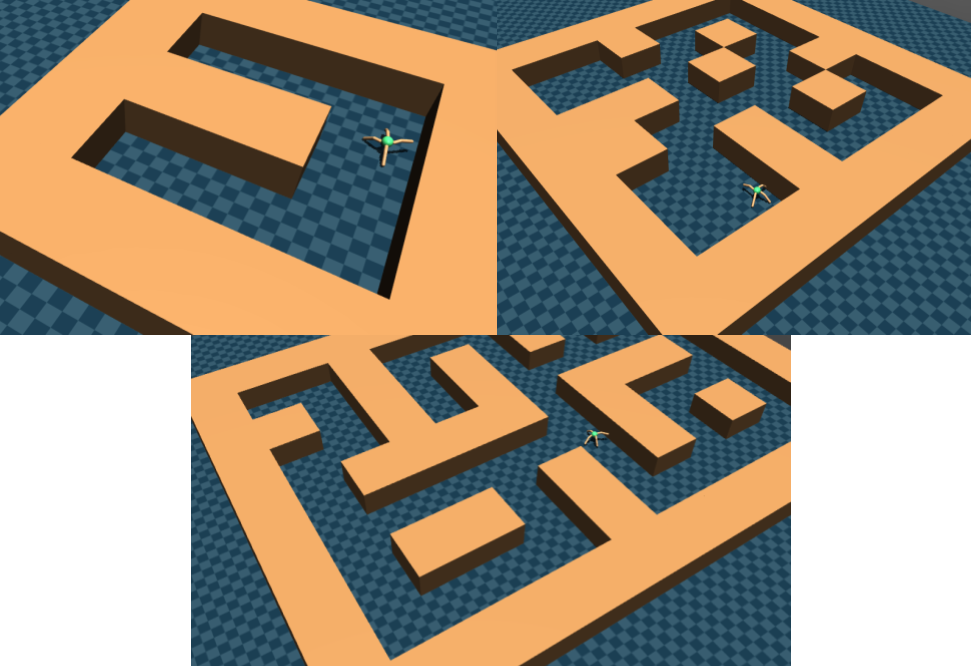
\includegraphics[width=0.17\textwidth]{chapters/cql/images/antmaze_all.png}
%     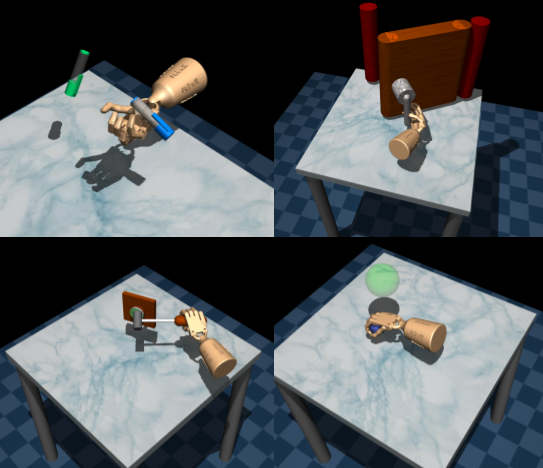
\includegraphics[width=0.97\linewidth]{chapters/cql/images/adroit_all.png}
%   \end{center}
%   \vspace{-21pt}
% \end{wrapfigure}
\textbf{Gym domains\footnote{An earlier version of the paper had results corresponding to \texttt{v0} versions of the D4RL benchmark from May 2020. Since then, D4RL has performed several modifications with respect to terminal/timeout handling and the latest release of D4RL is the v2 release. To facilitate comparisons on the latest version of the D4RL benchmark, we provide results with the \texttt{-v2} domains now.}} Results for the gym domains are shown in Table~\ref{table:mujoco}. The results for BEAR, BRAC, SAC, and BC are based on numbers reported by \citet{d4rl}. We find that across the board, on both the datasets generated by a single mediocre policy, marked as ``-medium'' and the datasets generated by mixing together experience from multiple policies (``-medium-replay'' and ``-medium-expert''), that are more likely to be encountered in practical problems, CQL outperforms prior methods.

% While CQL performs similarly to the best performing prior method when the offline dataset is constructed from a single RL policy, it significantly outperforms prior methods with complex data distributions, which are more indicative of real-world offline datasets~\citep{d4rl}.
%%SL.5.11: Well, if we're not going to show any of the AlgeaDICE results, maybe we shouldn't mention it before like this? We could add a sentence to the end of the first paragraph that describes all the prior methods and say something like: We also ran AlgeaDICE~\citep{} using code released by the authors, but were unable to get this method to improve over a random initialization on any of the tasks, as learning was unstable and diverged quickly.
% done
%%SL.5.11: In general, I think it would be best to break up the reported results into groups, and present them more slowly. For example, we could write the above paragraph something like this:
%The final performance of CQL($\mathcal{H}$) and each prior method on the D4RL tasks is shown in Table~\ref{table:something}. The first group of results is based on single-policy datasets for the MuJoCo gym benchmark environments: the ``-random'' and ``-medium'' datasets for HalfCheetah, Walker2D, and Hopper. These datsets are produced by either a random policy, or a medium-reward policy, respectively (see \citet{d4rl} for details). On these single-policy datasets, CQL matches or exceeds the best prior methods, but by a small margin. However, on the datasets that combine multiple policies (``-mixed,'' ``medium-expert,'' ``-random-expert''), prior methods generally perform substantially worse. Such mixed datasets are likely to be more common in real-world applications of offline RL, where training data might come from a variety of sources. CQL outperforms prior methods in these settings, on all three environments, in some cases by as much as 2-4x.
%%SL.5.11: You might want to also group the results in the tables/plots based on these groupings


% & halfcheetah-random & 100.0 & 2.1 & 30.5 & 25.5 & 23.5 & 28.1\\
% & walker2d-random & 100.0 & 1.6 & 4.1 & 6.7 & 0.8 & 0.5\\
% & hopper-random & 100.0 & 9.8 & 11.3 & 9.5 & 11.1 & 12.0\\
% & halfcheetah-medium & 100.0 & 36.1 & -4.3 & 38.6 & 44.0 & 45.5\\
% & walker2d-medium & 100.0 & 6.6 & 0.9 & 33.2 & 72.7 & 81.3\\
% & hopper-medium & 100.0 & 29.0 & 0.8 & 47.6 & 31.2 & 32.3\\
% & halfcheetah-medium-replay & 100.0 & 38.4 & -2.4 & 36.2 & 45.6 & 45.9\\
% & walker2d-medium-replay & 100.0 & 11.3 & 1.9 & 10.8 & -0.3 & 0.9\\
% & hopper-medium-replay & 100.0 & 11.8 & 3.5 & 25.3 & 0.7 & 0.8\\
% & halfcheetah-medium-expert & 100.0 & 35.8 & 1.8 & 51.7 & 43.8 & 45.3\\
% & walker2d-medium-expert & 100.0 & 6.4 & -0.1 & 26.0 & 3.1 & 66.6\\
% & hopper-medium-expert & 100.0 & 111.9 & 1.6 & 4.0 & 1.1 & 0.8\\
% %%%%%%%%%%%%%% TABLE %%%%%%%%%%%%%%%%%%%%%%
% \begin{table*}[h]
% \centering
% \small
% \begin{tabular}{l|r|r|r|r|r|r||r}
% \hline
% \textbf{Task Name} & \textbf{BC} & \textbf{SAC} & \textbf{BCQ} & \textbf{BEAR} & \textbf{BRAC-p} & \textbf{BRAC-v} & \textbf{CQL($\mathcal{H}$)}\\ \hline
% halfcheetah-random & -17.9 & 3502.0 & -2.1 & 2885.6 & 2641.0 & 3207.3 & \textbf{4524.7} \\
% halfcheetah-medium &  4196.4 & -808.6 & 4117.0 & 4508.7 & \textbf{5178.2} & \textbf{5365.3} & \textbf{5281.6} \\
% halfcheetah-mixed &  4492.1 & -581.3 & 3377.2 & 4211.3 & \textbf{5384.7} & \textbf{5413.8} & \textbf{5476.3}\\
% halfcheetah-medium-expert &  4169.4 & -55.7 &  7415.6 & 6132.5 & 5156.0 & 5342.4 & \textbf{9025.0}\\
% halfcheetah-random-expert &  -113.1 & 6298.7 & 7161.3 & 2768.8 & 3465.2 & -9.55 & \textbf{7951.9}\\ 
% \hline
% walker2d-random & 73.0 & 192.0 & 266.9 & 307.6 & 38.4 & 23.9 & \textbf{323.1}\\
% walker2d-medium & 304.8 & 44.2 & 881.7 & 1526.7 & 3341.1 & \textbf{3734.4} & \textbf{3801.4} \\
% walker2d-mixed & 518.6 & 87.8 & 384.6 & 495.3 & -11.5 & 44.5 & \textbf{1391.0} \\
% walker2d-medium-expert & 297.0 & -5.1 & 876.7 & 1193.6 & 141.7 & 3058.9 & \textbf{4348.1} \\
% walker2d-random-expert & 33.5 & 37.1 &  & 88.9 & 12.1 & 124.9 & \textbf{4245.8} \\
% \hline
% hopper-random & 299.4 & 347.7 & 274.7 & 289.5 & \textbf{341.0} & \textbf{370.5} & \textbf{355.2} \\
% hopper-medium & 923.5 & 5.7 & 1186.7 & 1527.9 & 994.8 & 1030.0 & \textbf{2403.1}\\
% hopper-mixed & 364.4 & 93.3 & 491.3 & 802.7 & 2.0 & 5.3 & \textbf{2267.9}\\
% hopper-medium-expert & \textbf{3621.2} & 32.9 & 2146.8 & 109.8 & 16.0 & 5.1 & \textbf{3699.1}\\
% \hline
% % ant-random & & & & & & & 932.4\\
% % ant-medium & & & & & & & 3325.4 \\
% % ant-mixed & & & & & & & 2973.8\\
% % ant-medium-expert & & & & & & & 3400.1 \\
% % ant-random-expert & & & & & & & 2309.3\\
% % \hline
% \end{tabular}
% \caption{{\footnotesize Performance of CQL and prior methods on gym MuJoCo tasks from D4RL. Observe that CQL performs similarly to the best prior method with simple datasets generated from a single RL policy, and greatly outperforms prior methods with mixed datasets.}}
% \label{table:mujoco}
% \normalsize
% \end{table*}
% %%SL.5.11: Maybe show some pictures of these tasks and the adroit and maze tasks, for readers that aren't familiar?
% % Yes I can add these, but i am concerned about too much space utilization
%%%%%%%%%%%%%%%%%%%%%%%%%%%%
% \begin{figure*}
% \centering
% 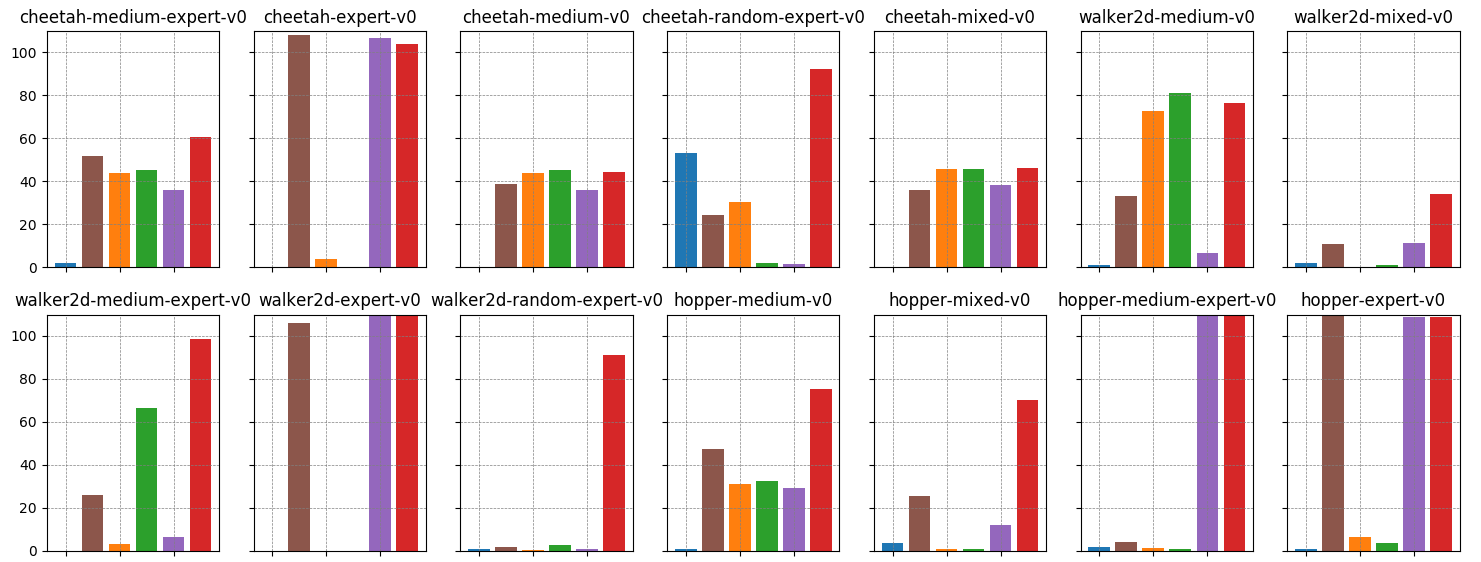
\includegraphics[width=0.99\linewidth]{chapters/cql/images/mujoco_results_v1.png}
% \caption{{\footnotesize Performance of CQL and prior methods on gym MuJoCo tasks from D4RL reported as a normalized score. Observe that CQL performs similarly to the best prior method with simple datasets generated from a single RL policy, and greatly outperforms prior methods with mixed datasets.}}
% \end{figure*}
    % 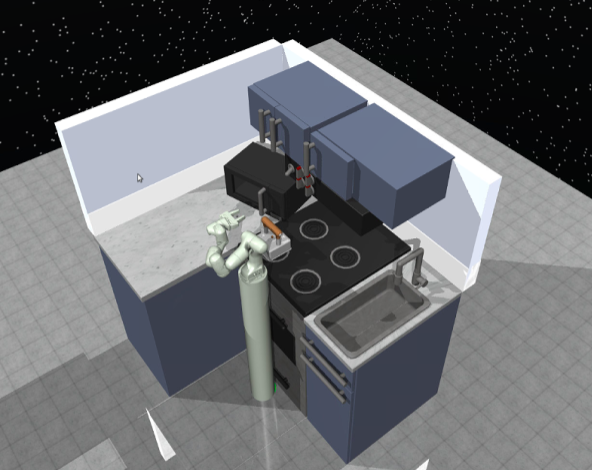
\includegraphics[width=0.9\linewidth]{chapters/cql/images/adept_franka_kitchen.png}

%% adroit tasks
\textbf{Adroit tasks.} The more complex Adroit~\citep{rajeswaran2018dapg} tasks in D4RL require controlling a 24-DoF robotic hand, using limited data from human demonstrations. These tasks are
substantially more difficult than the gym tasks in terms of both the dataset composition and high dimensionality. Prior offline RL methods generally struggle to learn meaningful behaviors on 
these tasks, and the strongest baseline is BC. As shown in Table~\ref{table:adroit_antmaze}, CQL variants are the only methods that improve over BC, attaining scores that are \textbf{2-9x} those of the next best offline RL method. CQL($\rho$) with $\rho = \hat{\policy}^{k-1}$ (the previous policy) outperforms CQL($\mathcal{H}$) on a number of these tasks, due to the higher action dimensionality resulting in higher variance for the CQL($\mathcal{H}$) importance weights. Both variants outperform prior methods.
%%AK.5.23: need to say something about the CQL(rho) variant doing better -- which is due to importance sampling, but we never really talk about importance sampling so far.

\begin{table}[H]
\captionsetup{font=small}
\vspace{-5pt}
\centering
%\scriptsize
\fontsize{8}{8}\selectfont
\begin{tabular}{l|l|r|r|r|r|r||r|r}
\hline
\textbf{Domain} & \textbf{Task Name} & \textbf{BC} & \textbf{SAC} & \textbf{BEAR} & \textbf{BRAC-p} & \textbf{BRAC-v} & \textbf{CQL($\mathcal{H}$)} & \textbf{CQL($\rho$)}\\ \hline
% \multirow{3}*{Maze2D}
% & maze2d-umaze &  3.8 & 88.2 & 3.4 & 4.7 & -14.6\\
% & maze2d-medium &  30.3 & 26.1 & 29.0 & 32.4 & 149.0\\
% & maze2d-large &  5.0 & -1.9 & 4.6 & 10.4 & 150.0\\
% \hline
\multirow{6}*{AntMaze}
& antmaze-umaze-v2 & 54.6 & 0.0 & {73.0} & 50.0 & 70.0 & \textbf{94.0} & - \\
& antmaze-umaze-diverse-v2  & 45.6 & 0.0 & 61.0 & 40.0 & 70.0 & {47.3} & - \\
& antmaze-medium-play-v2  & 0.0 & 0.0 & 0.0 & 0.0 & 0.0 & \textbf{62.4} & - \\
& antmaze-medium-diverse-v2  & 0.0 & 0.0 & 8.0 & 0.0 & 0.0 & \textbf{74.3}  & - \\
& antmaze-large-play-v2 & 0.0 & 0.0 & 0.0 & 0.0 & 0.0 & \textbf{34.2} & - \\
& antmaze-large-diverse-v2 & 0.0 & 0.0 & 0.0 & 0.0 & 0.0 & \textbf{40.7} & - \\
\hline
& \textbf{Total (antmazes)} & 100.2 & 0.0 & - & - & - & \textbf{352.9} & -\\
\hline
\multirow{8}*{Adroit}
& pen-human  & 34.4 & 6.3 & -1.0 & 8.1 & 0.6 & 37.5 & \textbf{55.8}\\
& hammer-human & 1.5 & 0.5 & 0.3 & 0.3 & 0.2 & \textbf{4.4} & {2.1}\\
& door-human & 0.5 & 3.9 & -0.3 & -0.3 & -0.3 & \textbf{9.9} & \textbf{9.1} \\
& relocate-human & 0.0 & 0.0 & -0.3 & -0.3 & -0.3 & 0.20 & \textbf{0.35}\\
& pen-cloned  & \textbf{56.9} & 23.5 & 26.5 & 1.6 & -2.5 & 39.2 & 40.3\\
& hammer-cloned & 0.8 & 0.2 & 0.3 & 0.3 & 0.3 & 2.1 & \textbf{5.7} \\
& door-cloned & -0.1 & 0.0 & -0.1 & -0.1 & -0.1 & 0.4 & \textbf{3.5}\\
& relocate-cloned & \textbf{-0.1} & -0.2 & -0.3 & -0.3 & -0.3 & \textbf{-0.1} & \textbf{-0.1}\\
\hline
\multirow{3}*{Kitchen}
& kitchen-complete & 33.8 & 15.0 & 0.0 & 0.0 & 0.0 & \textbf{43.8} & 31.3\\
& kitchen-partial & 33.8 & 0.0 & 13.1 & 0.0 & 0.0 & \textbf{49.8} & \textbf{50.1} \\
& kitchen-undirected & 47.5 & 2.5 & 47.2 & 0.0 & 0.0 & \textbf{51.0} & \textbf{52.4} \\ \hline
\end{tabular}
\vspace{0.1cm}
\caption{\label{table:adroit_antmaze}{Normalized scores of all methods on AntMaze, Adroit, and kitchen domains from D4RL, averaged across 4 seeds. On the harder mazes, CQL is the \textit{only} method that attains non-zero returns, and is the only method to outperform simple behavioral cloning on Adroit tasks with human demonstrations.
We observed that the CQL($\rho$) variant, which avoids importance weights, trains more stably, with no sudden fluctuations in policy performance over the course of training, on the higher-dimensional Adroit tasks.}}
\normalsize
\vspace{-22pt}
\end{table}

\textbf{AntMaze.\footnote{The results here use \texttt{antmaze-*-v2}. The original results from the 2020 version are shown in Appendix~\ref{sec:old_results}.}} 
These D4RL tasks require composing parts of suboptimal trajectories to form more optimal policies for reaching goals on a MuJoco Ant robot. 
Prior methods make some progress on the simpler U-maze, but only CQL is able to make meaningful progress  
%% adroit tasks
on the much harder medium and large mazes, outperforming prior methods by a wide margin.
%, achieving nearly \textbf{2-5x} higher return as compared to prior methods.

\begin{wrapfigure}{r}{0.15\textwidth}
  \vspace{-25pt}
  \begin{center}
  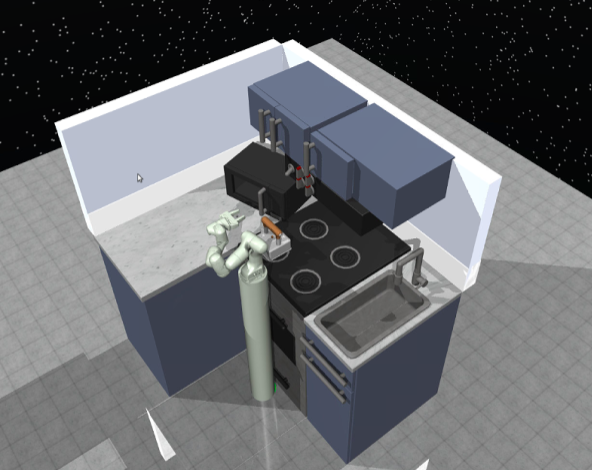
\includegraphics[width=0.99\linewidth]{chapters/cql/images/adept_franka_kitchen.png}
  \end{center}
  \vspace{-20pt}
\end{wrapfigure}
\textbf{Kitchen tasks.} Next, we evaluate CQL on the Franka kitchen domain~\citep{gupta2019relay} from D4RL~\citep{d4rl_repo}.
The goal is to control a 9-DoF robot to manipulate multiple objects (microwave, kettle, etc.) \textit{sequentially}, in a single episode to reach a desired configuration, with only sparse 0-1 completion reward for every object that attains the target configuration. These tasks are especially challenging, since they require composing parts of trajectories, precise long-horizon manipulation, and handling human-provided teleoperation data. As shown in Table~\ref{table:adroit_antmaze}, CQL outperforms prior methods in this setting, and is the only method that outperforms behavioral cloning, attaining over \textbf{40\%} success rate on all tasks.



% \begin{table*}[h]
% \centering
% \small
% \begin{tabular}{l|r|r|r|r|r|r|r|r}
% \hline
% \textbf{Task Name} & \textbf{SAC} & \textbf{BC} & \textbf{SAC-off} & \textbf{BEAR} & \textbf{BRAC-p} & \textbf{BRAC-v} & \textbf{CQL($\mathcal{H}$)} & \textbf{CQL($\rho$)}\\ \hline
% ant-umaze & 0.0 & 0.7 & 0.0 & 0.7 & 0.5 & 0.7 & \textbf{0.74} & \\
% ant-umaze-diverse & 0.0 & 0.6 & 0.0 & 0.6 & 0.4 & 0.7 & \textbf{0.79} & \\
% ant-medium-play & 0.0 & 0.0 & 0.0 & 0.0 & 0.0 & 0.0 & \textbf{0.54 } & \\
% ant-medium-diverse & 0.0 & 0.0 & 0.0 & 0.0 & 0.0 & 0.0 & \textbf{0.53} & \\
% ant-large-play & 0.0 & 0.0 & 0.0 & 0.0 & 0.0 & 0.0 & \textbf{0.20} & \\
% ant-large-diverse & 0.0 & 0.0 & 0.0 & 0.0 & 0.0 & 0.0 & \textbf{0.19} & \\
% \hline
% pen-human & 739.3 & 1121.9 & 284.8 & 66.3 & 339.0 & 114.7 & \textbf{1367.5} & \\
% hammer-human & -248.7 & -82.4 & -214.2 & -242.0 & -239.7 & -243.8 & \textbf{1098.1} & \\
% door-human & -61.8 & -41.7 & 57.2 & -66.4 & -66.5 & -66.4 & \textbf{273.0} & \\
% relocate-human & -13.7 & -5.6 & -4.5 & -18.9 & -19.7 & -19.7 & \textbf{5.7} & \\
% pen-cloned & \\
% hammer-cloned & \\
% door-cloned & \\
% relocate-cloned & \\
% \hline
% mini-kitchen-MKLS & \\
% kitchen-MKLS & \\
% kitchen-MKBL & \\
% \hline
% \end{tabular}
% \caption{{\footnotesize Performance of CQL and prior methods on AntMaze, Adroit and kitchen tasks from D4RL. Observe that CQL outperforms prior methods on the simpler U-shaped maze and is the \textit{only} method that is able to obtain non-zero performance on the harder, medium-sized maze. CQL is the only method that achieves a positive return on adroit tasks with human demonstrations.}}
% \label{table:adroit_antmaze}
% \normalsize
% \end{table*}
% \multirow{12}*{Adroit}
% & pen-human & 739.3 & 1121.9 & 284.8 & 66.3 & 339.0 & 114.7\\
% & pen-cloned & 739.3 & 1791.8 & 797.6 & 885.4 & 143.4 & 22.2\\
% & pen-expert & 739.3 & 2633.7 & 277.4 & 3254.1 & -7.8 & 6.4\\
% & hammer-human & -248.7 & -82.4 & -214.2 & -242.0 & -239.7 & -243.8\\
% & hammer-cloned & -248.7 & -175.1 & -244.1 & -241.1 & -236.7 & -236.9\\
% & hammer-expert & -248.7 & 16140.8 & 3019.5 & 16359.7 & -241.4 & -241.1\\
% & door-human & -61.8 & -41.7 & 57.2 & -66.4 & -66.5 & -66.4\\
% & door-cloned & -61.8 & -60.7 & -56.3 & -60.9 & -58.7 & -59.0\\
% & door-expert & -61.8 & 969.4 & 163.8 & 2980.1 & -66.4 & -66.6\\
% & relocate-human & -13.7 & -5.6 & -4.5 & -18.9 & -19.7 & -19.7\\
% & relocate-cloned & -13.7 & -10.1 & -16.1 & -17.6 & -19.8 & -19.4\\
% & relocate-expert & -13.7 & 4289.3 & -18.2 & 4173.8 & -20.6 & -21.4\\
% \hline
% \multirow{12}*{Gym}
% & halfcheetah-random & 12135.0 & -17.9 & 3502.0 & 2885.6 & 2641.0 & 3207.3\\
% & halfcheetah-medium & 12135.0 & 4196.4 & -808.6 & 4508.7 & 5178.2 & 5365.3\\
% & halfcheetah-mixed & 12135.0 & 4492.1 & -581.3 & 4211.3 & 5384.7 & 5413.8\\
% & halfcheetah-medium-expert & 12135.0 & 4169.4 & -55.7 & 6132.5 & 5156.0 & 5342.4\\
% & walker2d-random & 4592.3 & 73.0 & 192.0 & 307.6 & 38.4 & 23.9\\
% & walker2d-medium & 4592.3 & 304.8 & 44.2 & 1526.7 & 3341.1 & 3734.4\\
% & walker2d-mixed & 4592.3 & 518.6 & 87.8 & 495.3 & -11.5 & 44.5\\
% & walker2d-medium-expert & 4592.3 & 297.0 & -5.1 & 1193.6 & 141.7 & 3058.9\\
% & hopper-random & 3234.3 & 299.4 & 347.7 & 289.5 & 341.0 & 370.5\\
% & hopper-medium & 3234.3 & 923.5 & 5.7 & 1527.9 & 994.8 & 1030.0\\
% & hopper-mixed & 3234.3 & 364.4 & 93.3 & 802.7 & 2.0 & 5.3\\
% & hopper-medium-expert & 3234.3 & 3621.2 & 32.9 & 109.8 & 16.0 & 5.1\\
% \hline

%%SL.5.24: Consider deleting subsection headings in the whole experiments section. They really don't add much, and you can save some space.
%\subsection{Offline Image-Based RL on the Arcade Learning Environment}
\textbf{Offline RL on Atari games\footnote{Results for CQL on more Atari games, with varied dataset compositions can be found in Appendix F of DR3 (Kumar et al. ICLR 2022), available at the following arXiv URL: \url{https://arxiv.org/abs/2112.04716}}.} Lastly, we evaluate a discrete-action Q-learning variant of CQL (Algorithm~\ref{alg:practical_alg}) on offline, image-based Atari games~\citep{bellemare2013arcade}. We compare CQL to REM~\citep{agarwal2019optimistic} and QR-DQN~\citep{dabney2018distributional} on the five Atari tasks (Pong, Breakout, Qbert, Seaquest and Asterix) that are evaluated in detail by \citet{agarwal2019optimistic}, using the dataset released by the authors. 
% We were not able to reproduce the QR-DQN and REM results on Asterix using the official implementation and data from \citet{agarwal2019optimistic}, and no method was able to perform well on the provided data for this task, but we include the scores in Table~\ref{table:atari_reduced_size}.

\begin{figure*}[h]
\vspace{-12pt}
\begin{center}
  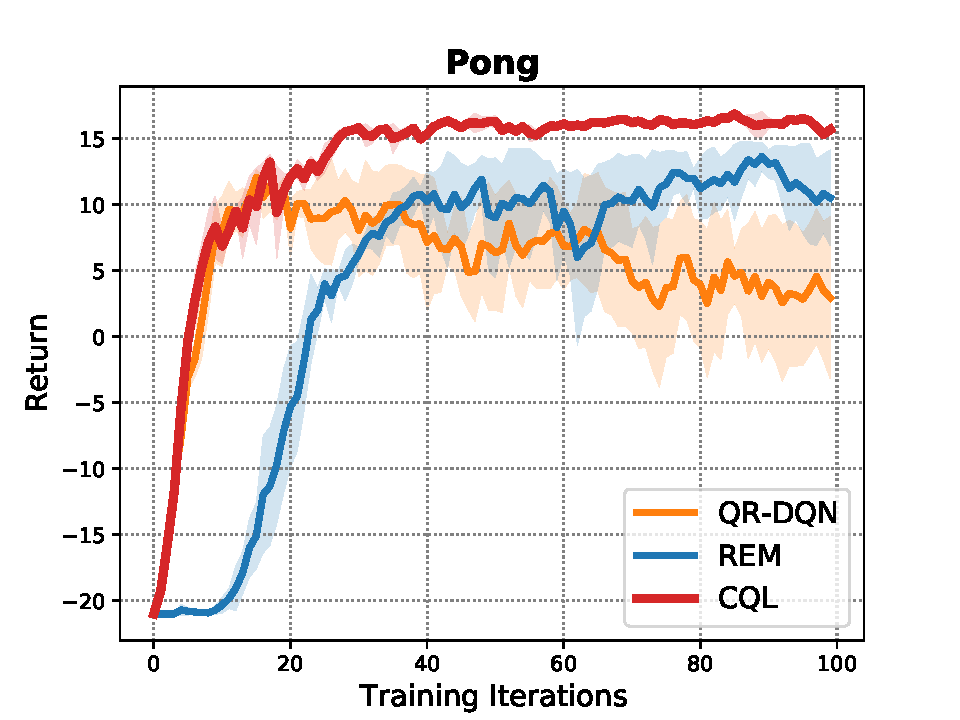
\includegraphics[width=0.23\linewidth]{chapters/cql/images/pong.pdf}  
  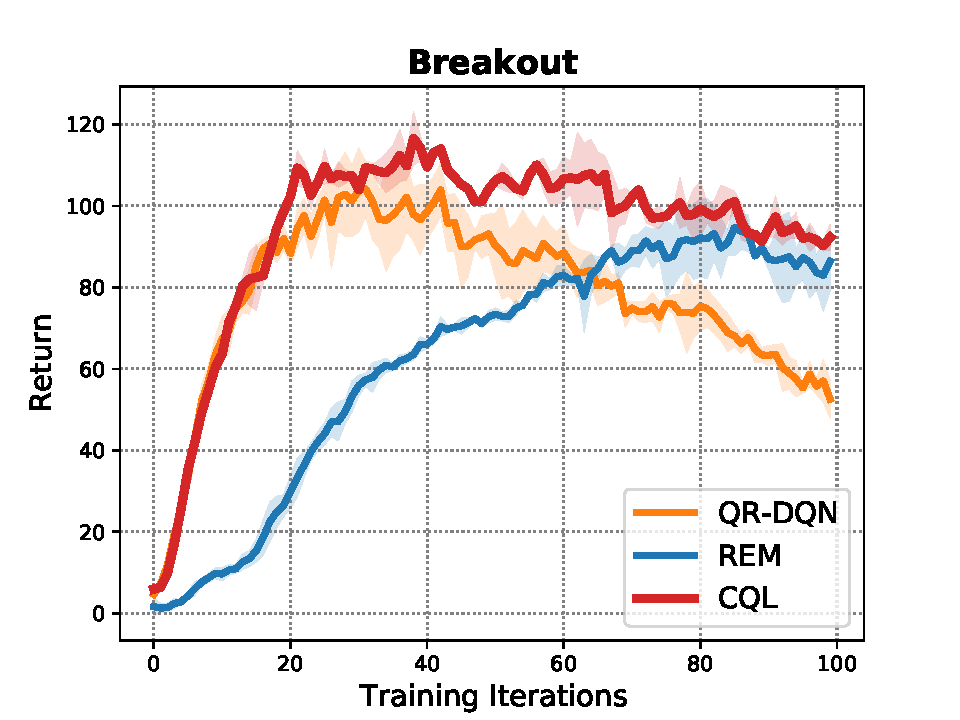
\includegraphics[width=.23\linewidth]{chapters/cql/images/breakout.pdf}  
  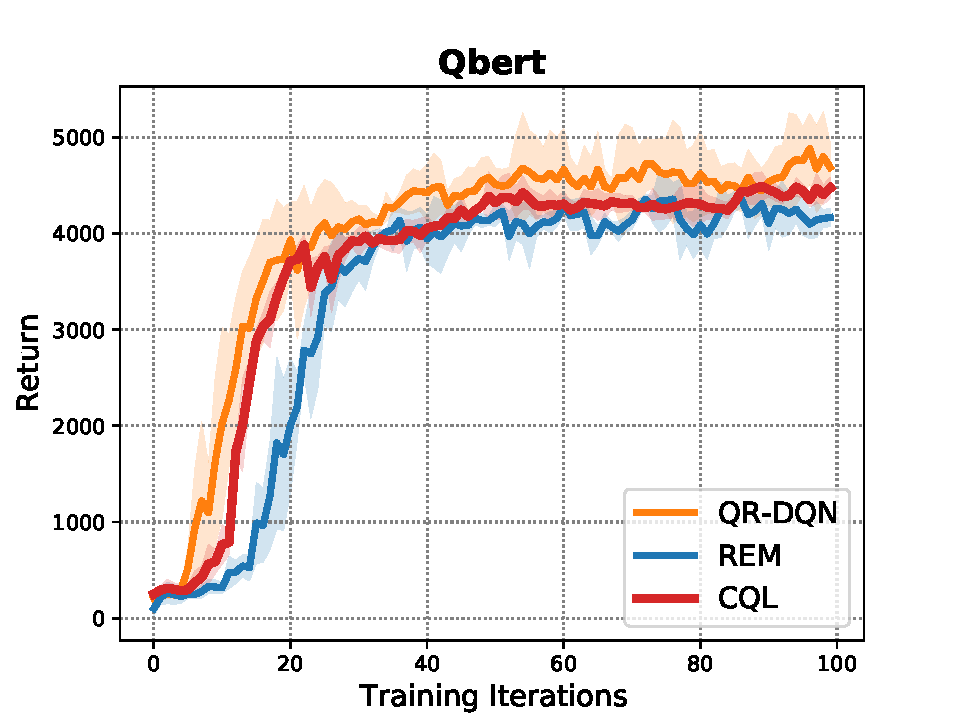
\includegraphics[width=.23\linewidth]{chapters/cql/images/qbert.pdf}  
  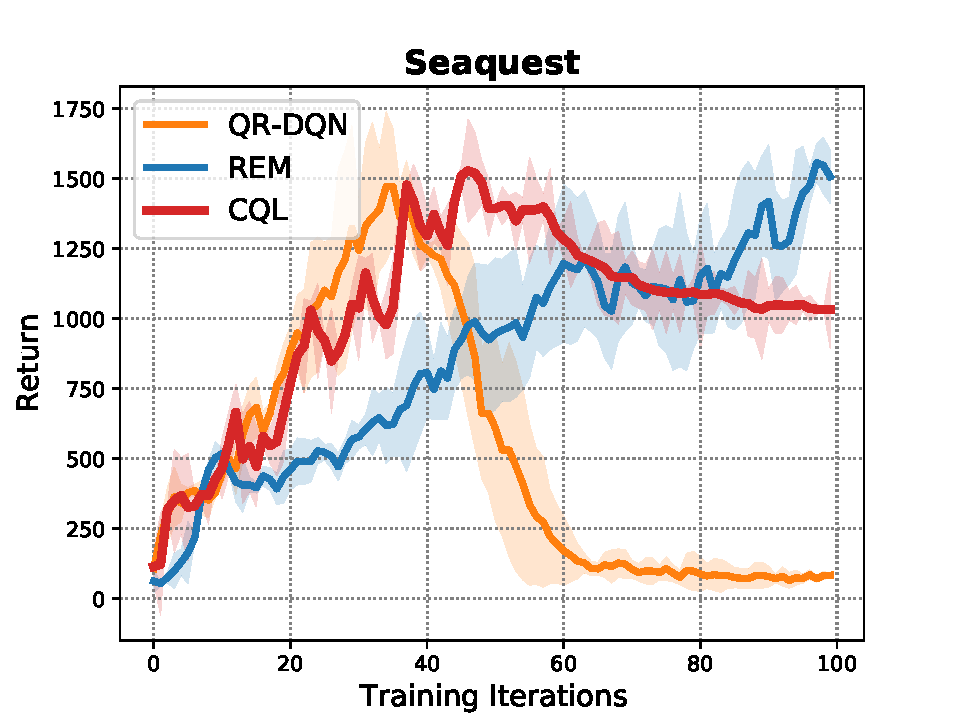
\includegraphics[width=.23\linewidth]{chapters/cql/images/seaquest.pdf}  
\end{center}
\vspace{-4pt}
\caption{\label{fig:cql_20m_atari}{\footnotesize Performance of CQL, QR-DQN and REM as a function of training steps (x-axis) in setting \textbf{(1)} when provided with only the first 20\% of the samples of an online DQN run. Note that CQL is able to learn stably on 3 out of 4 games, and its performance does not degrade as steeply as QR-DQN on Seaquest.}}
\vspace{-10pt}
\end{figure*}
Following the evaluation protocol of \citet{agarwal2019optimistic}, we evaluated on two types of datasets, both of which were generated from the DQN-replay dataset, released by~\citep{agarwal2019optimistic}:
\textbf{(1)} a dataset consisting of the first 20\% of the samples observed by an online DQN agent and 
\textbf{(2)} datasets consisting of only 1\%  and 10\% of all samples observed by an online DQN agent (Figures 6 and 7 in \citep{agarwal2019optimistic}). In setting \textbf{(1)}, shown in Figure~\ref{fig:cql_20m_atari}, CQL generally achieves similar or better performance throughout as QR-DQN and REM. When only using only 1\% or 10\% of the data, in setting \textbf{(2)} (Table~\ref{table:atari_reduced_size}),  CQL 
%AK: TODO (aviral): revisit this if we can't get seaquest to work -- Seaquest is almost maxed out, need to decide on what to say here?
\begin{wraptable}{r}{6.0cm}
\captionsetup{font=small}
    \centering
    \vspace{-7pt}
    \fontsize{8}{8}\selectfont
    \begin{tabular}{l|r|r||r}
    \hline
        \textbf{Task Name} & \textbf{QR-DQN} & \textbf{REM} & \textbf{CQL($\mathcal{H}$)} \\
        \hline
         Pong (1\%) & -13.8 & -6.9 & \textbf{19.3} \\
         Breakout & 7.9 & 11.0 & \textbf{61.1} \\
         Q*bert & 383.6 & 343.4 & \textbf{14012.0} \\
         Seaquest & 672.9 & 499.8 & \textbf{779.4} \\
         Asterix  & 166.3 & 386.5 & \textbf{592.4}\\
         \hline
         \hline
         Pong (10\%) & 15.1 & 8.9 & \textbf{18.5} \\
         Breakout & 151.2 & 86.7 & \textbf{269.3} \\
         Q*bert & 7091.3 & 8624.3 & \textbf{13855.6}\\
         Seaquest & 2984.8 & \textbf{3936.6} & 3674.1 \\
         Asterix & \textbf{189.2} & 75.1 & 156.3 \\
         \hline
    \end{tabular}
    \vspace{-4pt}
    \caption{{CQL, REM and QR-DQN in setting \textbf{(1)} with 1\% data (top), and 10\% data (bottom). CQL drastically outperforms prior methods with 1\% data, and usually attains better performance with 10\% data.}}
    \normalsize
    \label{table:atari_reduced_size}
    \vspace{-17pt}
\end{wraptable}
substantially outperforms REM and QR-DQN, especially in the harder 1\% condition, achieving \textbf{36x} and \textbf{6x} times the return of the best prior method on Q*bert and Breakout, respectively.
% \let\thefootnote\relax\footnote{{\small *Neither CQL nor any prior method, including REM, attains non-trivial performance on Asterix. When using exactly the same dataset and implementation provided by \citet{agarwal2019optimistic}, we were unable to reproduce the numbers reported in~\citep{agarwal2019optimistic} for QR-DQN and REM. }}

% \begin{table}[h]
% \captionsetup{font=small}
%     \centering
%     \vspace{-10pt}
%     \fontsize{8}{8}\selectfont
%     \begin{tabular}{l|r|r|r|||r|r|r}
%     \hline
%         \textbf{Task Name} & \textbf{QR-DQN} & \textbf{REM} & \textbf{CQL($\mathcal{H}$)}  & \textbf{QR-DQN} & \textbf{REM} & \textbf{CQL($\mathcal{H}$)}  \\
%         \hline
%          Pong & 3.0 & 6.0 & \textbf{19.3} & 16.7 & 16.8 & \textbf{18.5} \\
%          Breakout & 7.8 & 9.2 & \textbf{61.1} & 176.0 & 96.0 & \textbf{269.3} \\
%          Q*bert & 500.0 & 500.0 & \textbf{14012.0}& 11201.8 & 8070.2 & \textbf{13855.6}\\
%          Seaquest & 480.2 & 390.1 & \textbf{779.4} & 3300.0 & \textbf{4290.4} & 3674.1 \\
%          %%SL.5.30: Something is wrong! This footnote doesn't seem to actually show up in the paper!!
%          Asterix\footnote{No method (CQL or prior methods, REM and QR-DQN, were able to attain non-trivial performance on this game using the dataset provided by \citet{agarwal2019optimistic}} & 166.3 & 386.5 & \textbf{592.4} & 189.2 & 75.1 & 156.3 \\
%          \hline
%     \end{tabular}
%     \caption{{CQL, REM and QR-DQN in setting \textbf{(1)} with 1\% data (left), and 10\% data (right). CQL drastically outperforms prior methods with 1\% data, and usually attains better performance with 10\%.}}
%     \normalsize
%     \label{table:atari_reduced_size}
% \footnote{No method (CQL or prior methods, REM and QR-DQN, were able to attain non-trivial performance on this game using the dataset provided by \citet{agarwal2019optimistic}}
% \end{table}

\textbf{Analysis of CQL.} Finally, we perform empirical evaluation to verify that CQL indeed lower-bounds the value function, thus verifying Theorems~\ref{thm:cql_underestimates}, Appendix~\ref{thm:policy_eval_func_approx} empirically. To this end, we estimate the average value of the learned policy predicted by CQL, $\E_{\bs \sim \mathcal{D}}[\hat{V}^k(\bs)]$, and report the difference against the actual discounted return of the policy $\policy^{k}$ in Table~\ref{table:cql_lower_bound}. We also estimate these values for baselines, including the minimum predicted Q-value under an ensemble~\citep{haarnoja,fujimoto2018addressing}
%%SL.5.30: Maybe reference some papers that do this, like TD3 and REM?
of Q-functions with varying ensemble sizes, which is a standard technique to prevent overestimed Q-values~\citep{fujimoto2018addressing,haarnoja,hasselt2010double} and BEAR~\citep{kumar2019stabilizing}, a policy constraint method. The results show that CQL learns a lower bound for all three tasks, whereas the baselines are prone to overestimation. We also evaluate a variant of CQL that uses Equation~\ref{eqn:objective_1}, and observe that the resulting values are lower (that is, underestimate the true values) as compared to CQL($\mathcal{H}$). This provides empirical evidence that CQL($\mathcal{H}$) attains a tighter lower bound than the point-wise bound in Equation~\ref{eqn:objective_1}, as per Theorem~\ref{thm:cql_underestimates}. We also present an empirical analysis to show that Theorem~\ref{thm:gap_amplify}, that CQL is gap-expanding, holds in practice in Appendix~\ref{app:gap_amplify}, and present an ablation study on various design choices used in CQL in Appendix~\ref{app:additional_results}.

\begin{table}[h]
\captionsetup{font=small}
\centering
\vspace{-5pt}
    \fontsize{8}{8}\selectfont
    \begin{tabular}{l|r|r||r|r|r|r|r}
    \hline
        \textbf{Task Name} & \textbf{CQL($\mathcal{H})$} & \textbf{CQL (Eqn.~\ref{eqn:objective_1})} & \textbf{Ensemble(2)}  & \textbf{Ens.(4)} & \textbf{Ens.(10)} & \textbf{Ens.(20)} & \textbf{BEAR} \\
        \hline
        %%SL.5.30: bold the best result that is still a bound
        hopper-medium-expert & \textbf{-43.20} & -151.36 & 3.71e6 & 2.93e6 & 0.32e6 & 24.05e3 & 65.93 \\
        hopper-mixed & \textbf{-10.93} & -22.87 & 15.00e6 &  59.93e3 & 8.92e3 & 2.47e3 & 1399.46 \\
        hopper-medium & \textbf{-7.48} & -156.70 & 26.03e12 & 437.57e6 & 1.12e12 & 885e3 & 4.32 \\
        %%SL.5.30: I would recommend using scientific notation (e.g., e6 or $\times 10^6$) instead of "M" or "T"
        \hline
    \end{tabular}
    \caption{{Difference between predicted policy values and the true policy value for CQL, a variant of CQL that uses Equation~\ref{eqn:objective_1}, the minimum of an ensemble of varying sizes, and BEAR~\citep{kumar2019stabilizing} on three D4RL datasets. CQL is the only method that lower-bounds the actual return (i.e., has negative differences), and CQL($\mathcal{H})$ is much less conservative than CQL (Eqn.~\ref{eqn:objective_1}).}}
    \normalsize
    \vspace{-10pt}
    \label{table:cql_lower_bound}
\end{table}


%%AK.5.23: Commenting out this for now, discussion in the email. Basically we are not doing great here especially with the right way of using the Q-values for computing policy return. It is conservative, but it is too conservative in 4/8 cases (like the method outputs 153.4 as the return, but the actual return is 276). I think that if we believe that the other story is storng enough, we should probably not have it.
% \subsection{Off-Policy Evaluation Experiments}

% %%SL.5.11: Can we start off with a little transition to explain why we're talking about this? E.g., something like: The core of CQL is a Q-function learning method that learns a lower bound on the true Q-function. This lower bound can be used to learn a better policy, or simply to evaluate an existing policy. In this section, we study this latter setting, applying CQL to the off-policy evaluation problem.
% % done
% CQL learns a Q-function such that the expected value of the policy under this learned Q-function lower-bounds the true policy value. In this section, we evaluate the performance of CQL for evaluating the performance of a pre-specified policy using pre-specified offline datasets on three continuous control domains: Hopper, HalfCheetah and Walker2d. In accordance with the setup in prior work~\citep{Zhang2020GenDICE}, our task is to evaluate the return of an expert SAC policy using data generated from a mixture of suboptimal policies. Thus, we use the medium-expert and mixed datasets from \citep{d4rl} that contain a diverse mixture of suboptimal policies as the offline datasets.

% We compare CQL to state-of-the-art prior method, GenDICE~\citep{zhang2019generalized}, in Table ??. Note that CQL learns conservative return estimates, that lower bound the actual discounted return of the target policy, thus empirically validating the theoretical insights discussed in Section~\ref{sec:policy_eval}. In contrast,  (One line about OTHER METHODS once we have numbers) \ak{TODO: put table.}
